              %******************************************%
              %                                          %
              %         Standard thesis template         %
              %            by Stefano Bianchi            %
              %       translation by Simone Deiana       %
              %                                          %
              %          version: 27 June 2024           %
              %                                          %
              %******************************************%
       
% If one wants to print on both sides, substitute 'oneside' for 'twoside'
% in the parameters of \documentclass
\documentclass[a4paper,11pt,oneside,openany]{book}

\usepackage[english]{babel}

\usepackage[utf8]{inputenc} % Enables the use of accented Italian characters
\usepackage[T1]{fontenc} % Enables the use of special characters usually not present in English alphabets

\usepackage{fancyhdr} % Allows for the rendering of the cover

\usepackage{graphicx} % Allows for the inclusion of figures in the document
\usepackage{epigraph}
\usepackage{enumitem}
\usepackage{xcolor}
\usepackage{listings}
\definecolor{mygreen}{rgb}{0,0.6,0}
\definecolor{mygray}{rgb}{0.5,0.5,0.5}
\definecolor{mymauve}{rgb}{0.58,0,0.82}

\lstset{
	backgroundcolor=\color{white},   % Choose the background color
	basicstyle=\footnotesize\ttfamily, % Set the font style
	breakatwhitespace=false,         % Break lines only at white space
	breaklines=true,                 % Break long lines
	captionpos=b,                    % Position of caption (b: bottom)
	commentstyle=\color{gray},    % Custom color for comments
	keywordstyle=\color{blue},       % Custom color for keywords
	numberstyle=\tiny\color{mygray}, % Custom color for line numbers
	stringstyle=\color{mygreen},    % Custom color for strings
	frame=single,                    % Add a frame around the code
	keepspaces=true,                 % Keep spaces in text
	language=Java,                   % Specify the programming language
	numbers=left,                    % Show line numbers on the left
	showspaces=false,                % Don't show spaces
	showstringspaces=false,          % Don't show spaces in strings
	showtabs=false,                  % Don't show tabs
	tabsize=2                        % Set tab size
}


\usepackage{subfigure} % Allows for the inclusion of subfigures in the document

\usepackage{tabularx} % Adds functionalities to tables
\usepackage{longtable} % Allows to write tables on multiple pages

\usepackage[titletoc]{appendix} % Allows to put appendix chapters in the index

\usepackage{float} % Needed to include floating images

\usepackage{fancyvrb} % Allows for the use of Verbatim windows (i.e. unformatted text) inside a frame

\usepackage{amsmath} % Adds functionalities to formulas
\numberwithin{equation}{section}

\usepackage{hyperref} % Index of the topics with clickable link, for a more comfortable document navigation

\usepackage{lipsum} % Allows for the insertion of filler text inside the thesis; useless when writing. Delete this command and all the \lorem commands inside the text.

% To add content, refer to the relative files marked by parenthesis in the parameters of \input

%*******************************************************
% Settings of the single page and the cover
%*******************************************************
\hypersetup{ % Visualization of clickable links
    colorlinks,
    citecolor=black,
    filecolor=black,
    linkcolor=black,
    urlcolor=black
}

% Sets the pages' header
\fancyhf{}
\pagestyle{fancy}
\lhead{}
\chead{\leftmark}
\rhead{}
\lfoot{}
\cfoot{}
%\rfoot{\thepage}

% Sets the page's numberings
\fancyfoot[C]{\thepage} % Center the page number with "Page" before it


%*******************************************************
% Cover
%*******************************************************
% Configures the cover
% Do not modify this part
\usepackage[some]{background}
\SetBgScale{1}
\SetBgContents{

\includegraphics[scale=1]{img/units_logo.pdf}}
\SetBgColor{gray}
\SetBgAngle{0}
\SetBgOpacity{0.07}
% Do not modify this part

% Title of the thesis and name of the author
\title{Restoration and development of a web-based LEGv8 ISA simulator}
\author{Name Surname}
\begin{document}
\pagenumbering{roman}
\begin{titlepage}
    \begin{center}
    % Insert the background here (front page)
    \BgThispage
    {\LARGE {\bfseries UNIVERSITY OF TRIESTE \\}}
    \vspace{.5cm}
    {\Large {\bfseries Department of Engineering and Architecture \\}}
    \vspace{1cm}
    
\includegraphics[width=6cm,height=6cm]{img/units_logo.pdf}\\[1.5cm]

    {\LARGE
        Master's degree in Computer Engineering \\
    }
    \vspace{1cm}
    {\LARGE 
        {\bfseries Restoration and development of a web-based LEGv8 ISA simulator}
    }
    \vspace{1cm}

    % Remember to update the date before printing the document :)
    {\large \today \\
    }

    % Table to report the names of the graduating student, supervisor and co-supervisor (if present)
    \vfill
    \begin{table}[h]
        {\large
            \begin{tabular}{c c c c r c c | c c l}
                & & & & Graduating student & & & & & Supervisor \\
                & & & & \bfseries Simone Deiana & & & & & \bfseries Prof. Alberto Carini \\ % Modify the name of the graduating student
                & & & & & & & & & \\
            \end{tabular}
        }
    \end{table}
    Academic Year 2023/2024
    \end{center}
\end{titlepage}

	
\frontmatter

%*******************************************************
% Summary
%*******************************************************
\chapter{Summary}\label{chap:summ}

In this thesis I will be reporting my work done developing upon a Java-based LEGv8 ISA simulator.
\\

In the Introduction I will provide a brief overview of the LEGv8 ISA together with the reasons for choosing this thesis project in the context of the Digital Architectures course.
\\

In Chapter 1 I will provide a short summary of the current landscape of software simulators available online for the LEGv8 ISA. I will end the chapter with a focus on the simulator chosen for this thesis' project, namely the LEGv8 simulator developed and distributed by Arm Holdings plc. I will give an overview of its working state, functionality and structure prior to my development efforts.
\\

In Chapter 2 I will present the work done to decouple the project from the Eclipse IDE and migrate it to a modern build automation system, namely Maven.
\\

In the Chapter 3 I will showcase the bugs that have been fixed and I will introduce all of the functionalities that have been added to the simulator and the structural changes by them entailed.
\\

In Chapter 4 I will talk about the shortcomings of the simulator and the work that can be done to further improve it.

\newpage

%*******************************************************
% Index
%*******************************************************
\tableofcontents
\newpage

%*******************************************************
% Introduction
%*******************************************************
% Do not modify this part
\renewcommand{\chaptermark}[1]{\markboth{\MakeUppercase{\ #1}}{}}
% Do not modify this part

\chapter{Introduction}
% Fill with what you want to include in the introduction
\epigraph{``Simplicity is a great virtue but it requires hard work to achieve it and education to appreciate it. And to make matters worse: complexity sells better.''}{\textit{Edsger W. Dijkstra}}

\section*{What is an ISA?}

A computer is a device which is capable of acquiring data, performing calculations upon it, and making the results available for use at a later date.
It is clear from this definition, that when deciding how to design and build a computer one must at least take into consideration the way data is 
stored and organized (the memory) and the mechanisms through which the computer is able to manipulate said data (the processor).
Computers are an abstract concept and do not impose a certain technological choice to their physical realization. Nonetheless, the vast majority of computers nowadays
are built through the assembly of digital components and thus natively speak the language of the binary number system.
As such, just like when using a mechanical device an operator needs to interact with the physical parts of the system,  operating a computer at this level
would require the user to manually insert ones and zeros into the right places for it to perform its calculations.
It is clear that such an operation would require an intimate knowledge of the physical implementation of the computer, and even minimal
changes to its digital circuitry might jeopardize the correctness of any sequences of bits written for an earlier model.

Early on in the history of computers it was understood that an additional layer of abstraction was needed in order to separate the hardware from the software
and give more freedom both to the circuit designers and the programmers. This layer of abstraction is called an Instruction Set Architecture,
which from now on will be called ISA for short. An ISA provides a logical specification of how a computer manages its memory and what the instructions that it's
capable of performing are. This forms the layer through which all software must interface with in order to interact with the hardware.

\section*{What is the LEGv8 ISA?}

The ISA focus of this thesis is the LEGv8 ISA, an ARM-inspired architecture created by David A. Patterson and John L. Hennessy designed to serve as a teaching
tool in their book \emph{Computer Organization and Design (ARM Edition)}. As the title suggests, the book is actually about the ARMv8 ISA, whose first
iteration was originally released in 1983 by Acorn Computers and which is now developed by Arm Holdings plc. The authors, however, have introduced a few
changes and simplifications to the ARMv8 ISA to make it friendlier to students and emphasize certain design concepts. As such, this ISA is used
in the sections of the book dedicated to the design of a model processor and its programming, and it's these sections upon which the LEGv8 simulator
subject of this thesis is based.

\section*{Overview of the LEGv8 ISA}

\begin{figure}[H]
	\centering
	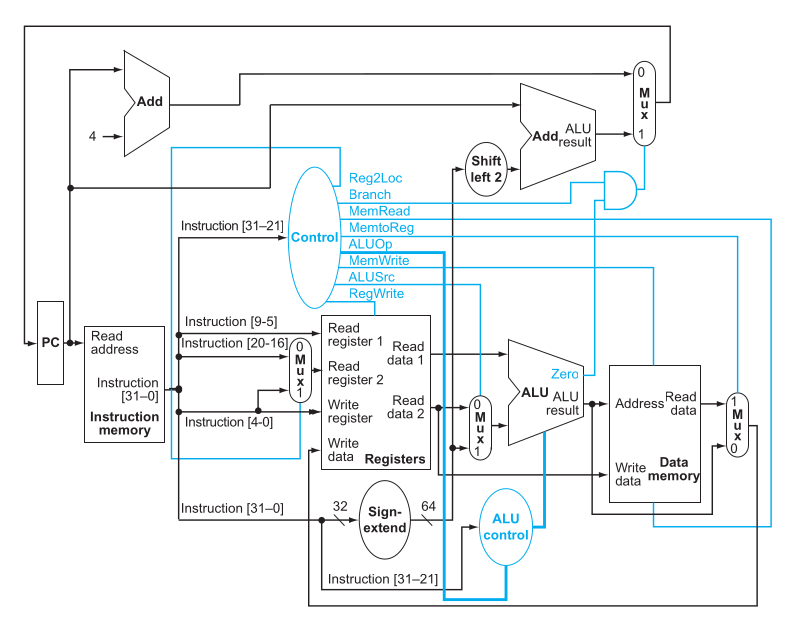
\includegraphics[width=.8\textwidth]{img/legv8_logical_scheme.png}
	\caption{The logical scheme of the LEGv8 architecture}
\end{figure}

\subsection*{Architecture type}
LEGv8 follows the Von Neumann architecture paradigm and thus contemplates the existence of a single memory containing both the instructions and the program data. It is a 64-bit architecture and is specifically designed for pipelined execution.
\subsection*{Registers}
LEGv8 defines 32 64-bit \emph{X} registers for storing integer values and 32 64-bit \emph{D} registers for storing double precision floating point values. There are also 32 32-bit \emph{S} registers dedicated to single precision floating point values, albeit being purely logical and simply occupying the lower 32 bits of the \emph{D} registers. Unlike ARMv8, the presence of 32-bit \emph{W} integer registers is not contemplated.
\newline
Registers are also used following a certain convention that is defined by the ISA but not enforced by the processor, and some can be addressed using alternative names for readibility purposes. There are analogous conventions for floating point registers too.
\begin{figure}[H]
	\centering
	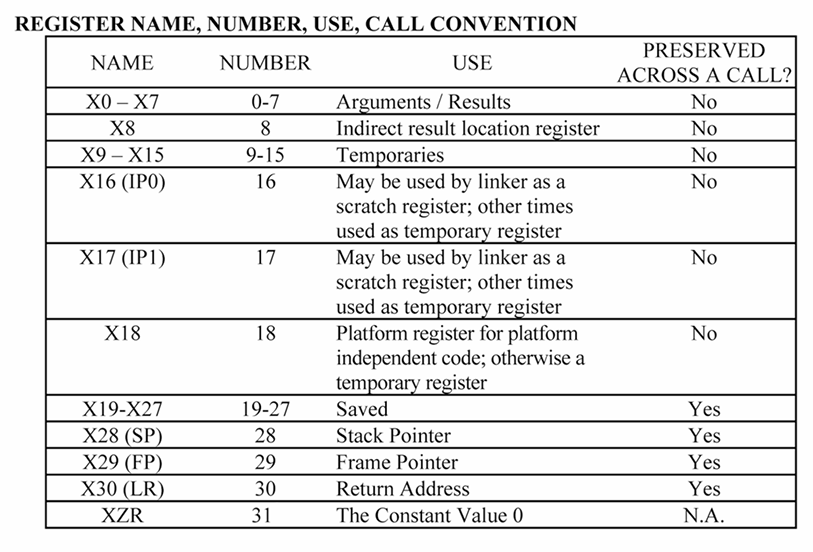
\includegraphics[width=.8\textwidth]{img/registers_conventions.png}
	\caption{Integer registers usage convention}
\end{figure}
\newline

In addition to the normal registers directly accessible by the programmer, more exist to store the program counter (i.e. the address of the current instruction to be executed) and various flags to keep track of overflows or carry bits in arithmetic operations and comparisons.
\subsection*{Memory}
The memory contains both the program code and the data. It is logically divided into a \emph{reserved} segment, a \emph{text} segment containing the program code, a \emph{static data} segment containing the constants defined at compile time, and a \emph{dynamic data} and \emph{stack} segments occupying the same location of memory and respectively growing upwards from the \emph{static data} segment and downwards from the stack pointer. This section of the memory is the one containing the data defined at execution time.
\begin{figure}[H]
	\centering
	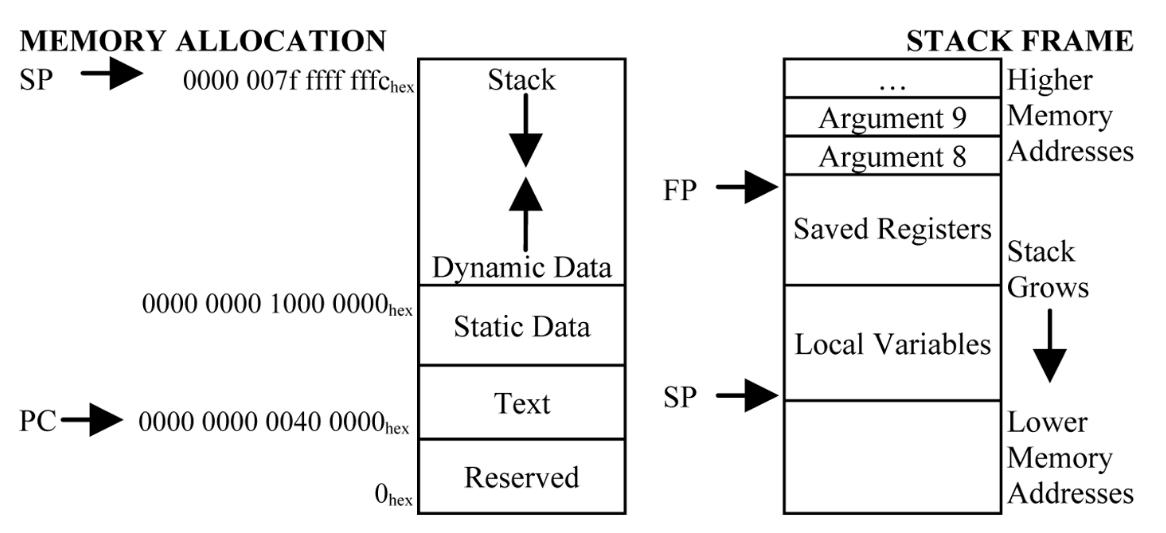
\includegraphics[width=.8\textwidth]{img/main_memory_layout.png}
	\caption{Logical division of the memory}
\end{figure}
\subsection*{Control unit}
The control unit is the component responsible for coordinating the pipeline execution flow and configuring the various components to perform the desired operations in the correct order using the correct parameters.
\subsection*{ALU}
The LEGv8 ALU is capable of performing 64-bit integer operations and both single and double precision floating point operations. The operation to perform at any given moment is configured through an ALUop code provided by the control unit.
\subsection*{Pipeline}
The LEGv8 pipeline is comprised of 5 stages: \emph{fetch}, \emph{decode}, \emph{execute}, \emph{data access}, and \emph{write back}.
As the names suggest, the \emph{fetch} stage is responsible for acquiring instructions from the text segment of the memory, the \emph{decode} stage decodes the instructions, reads the registers involved in the operation, and configures the control unit accordingly, the \emph{execute} stage performs the calculation through the ALU, the \emph{data access} stage is responsible for accessing the the memory, and the \emph{write back} stage finally writes the result into the registers.
Of course not all instructions make use of all the pipeline stages and this is taken into consideration when optimizing the execution flow.
\begin{figure}[H]
	\centering
	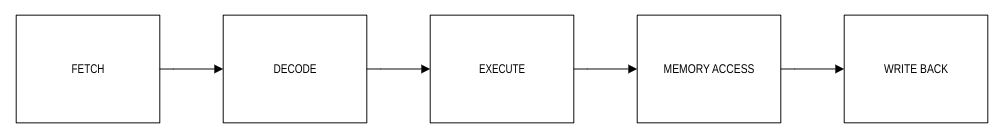
\includegraphics[width=.8\textwidth]{img/5_stage_pipeline.png}
	\caption{The 5 pipeline stages}
\end{figure}
\subsection*{Instructions}
LEGv8 can be considered a subset of ARMv8, but with a few caveats. Many higher level instructions have been omitted altogether in order to keep the ISA as minimal as possible, and many of the ones that have been kept have been revisited to make them clearer in their scope. For example, in ARMv8 the \emph{ADD} instruction can be used with both 32 and 64 bit integer registers, and both with register-based and immediate-based (i.e. defined directly in the program code) values. This of course allows the ARMv8 programmer to remember a single mnemonic and use it in all sorts of operations, but it obscures some important underlying design differences that might be valuable to computer architecture students. In LEGv8 instead, it has been decided to split the \emph{ADD} instruction into \emph{ADD} and \emph{ADDI} or register and immediate values usage respectively. Similarly, in ARMv8 the \emph{FADD} instruction is capable of performing additions both in the case of single and double precision registers, whereas in LEGv8 the instruction has been split into \emph{FADDS} and \emph{FADDD} for performing the operation only on single precision or double precision registers respectively.
\begin{figure}[H]
	\centering
	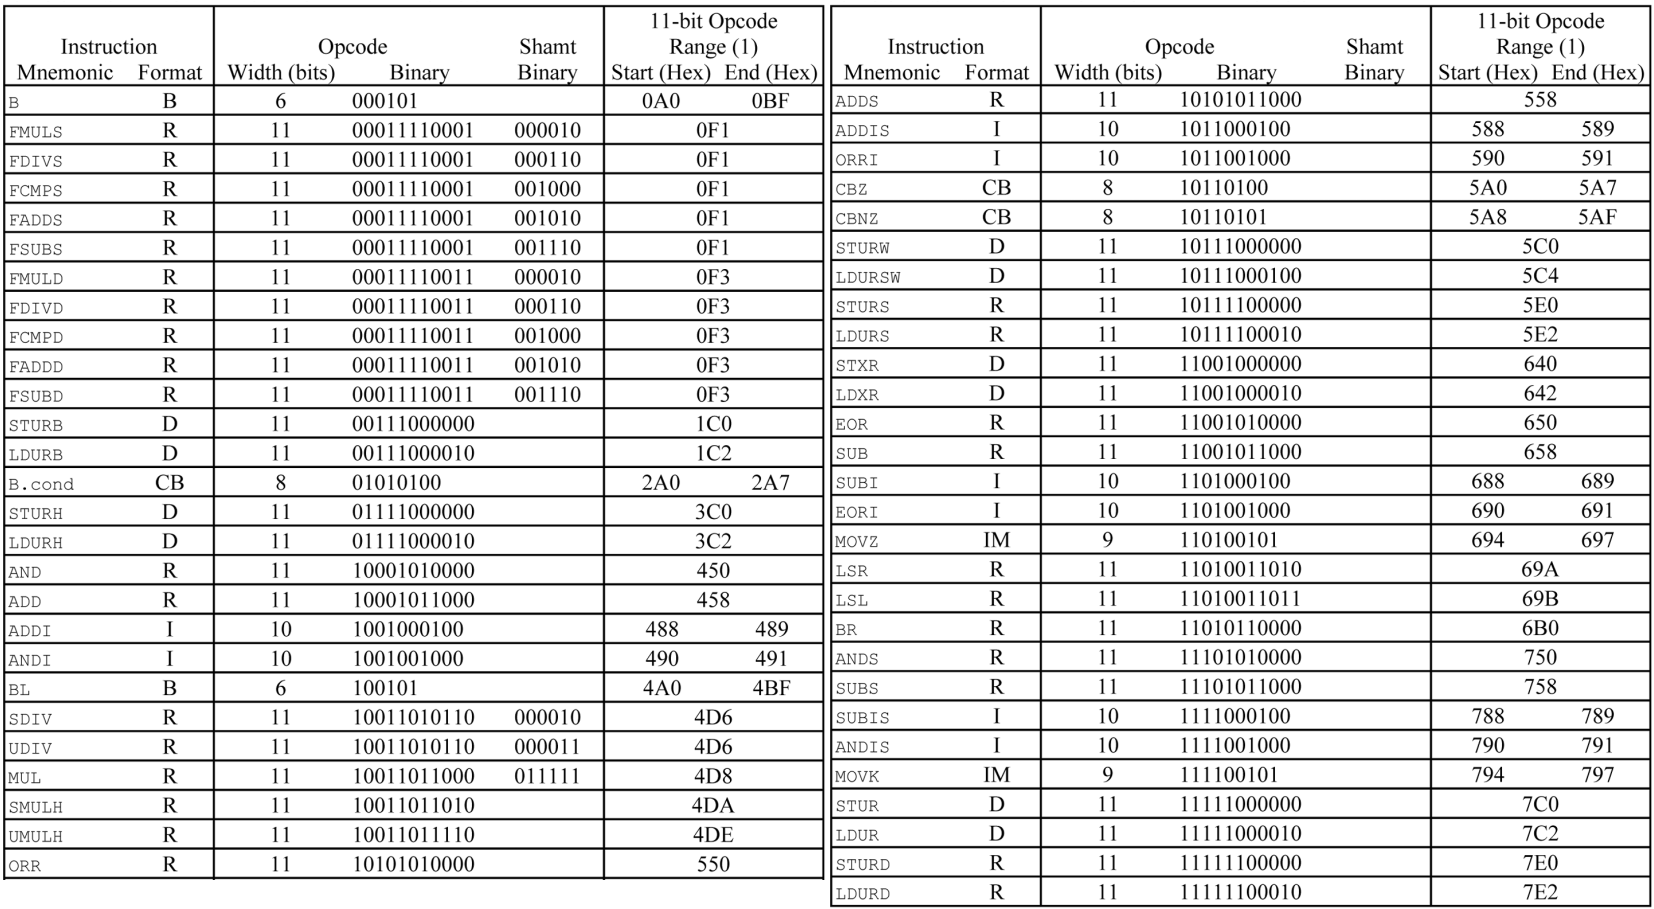
\includegraphics[width=.8\textwidth]{img/legv8_instruction_set.png}
	\caption{The complete LEGv8 ISA}
\end{figure}
All the instructions are encoded with the same length of 32 bits in order to fetch and decode them more efficiently. They are also grouped into 5 instruction formats to give a more homogeneous encoding to operations performing similar steps and increase their decoding speed.
The \emph{R}-type instructions perform operations solely on registers, the \emph{I}-type instructions make use of immediate values, the \emph{D}-type instructions access the memory, the \emph{B}-type and \emph{CB} perform unconditional and conditional branching respectively, and the \emph{IW}-type instructions to perform MOV instructions with wider immediate values.
\begin{figure}[H]
	\centering
	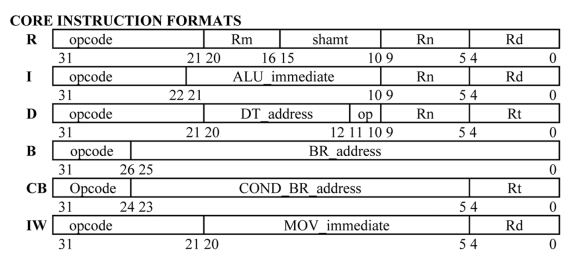
\includegraphics[width=.8\textwidth]{img/instruction_types.png}
	\caption{The 5 formats of LEGv8 instructions with their encoding pattern}
\end{figure}
\section*{Motivations for choosing LEGv8}
The LEGv8 ISA, being presented and defined in one of the major computer architecture undergraduate textbooks, is taught in many university courses around the world, including the Digital Systems Architecture course held by Prof. Carini at UniTS. In spite of its popularity, no real hardware has been made to run its instruction set natively, and the simulator landscape is almost equally lacking in viable options. This in turn makes it impossible for educators and students alike to show working examples of LEGv8 code, depriving them of teaching and learning opportunities. For these reasons I have chosen to work on an already existing and partially working LEGv8 simulator provided by Arm Holdings plc. to expand upon its functionalities to include a complete simulation of the ISA. 



\newpage

%*******************************************************
% Chapters
%*******************************************************
\mainmatter

% Do not modify this part
\renewcommand{\chaptermark}[1]{\markboth{\MakeUppercase{\chaptername\ \thechapter.\ #1}}{}}
% Do not modify this part

% Add all the necessary chapters. One can add all the chapters
% inside of a single .tex file or through one .tex file per chapter.

\chapter{The LEGv8 simulators landscape}

\epigraph{``It used to be the program's purpose to instruct our computers; it became the computer's purpose to execute our programs.''}{\textit{Edsger W. Dijkstra}}

The current landscape of publicly available LEGv8 simulators can be divided into two categories: simulators that aim to reproduce the logical design presented in the textbook in chapter 4, and the simulators providing a high level simulation of the instruction set as defined in the book.
The survey was performed on GitHub using ``LEGv8'' and ``simulator'' as keywords and only those in a reasonably working state (as per the author) have been considered.

\subsection*{Software simulators}

\begin{table}[H]
	\centering
	\resizebox{\textwidth}{40}{ \begin{tabular}{|c|c|c|c|c|c|c|}
		\hline
		\textbf{Repository} & \textbf{Language} & \textbf{Integer Support} & \textbf{Pipelined} & \textbf{Registers view} & \textbf{Stack view} & \textbf{Floating Point Support} \\
		\hline
		\url{https://github.com/lcpckp/leg-cpu-sim} & Java & Partial & No & Yes & Yes & No \\
		\hline
		\url{https://github.com/chrwoods/legv8-emul} & C/C++ & Partial & Yes & Yes & Yes & No \\
		\hline
		\url{https://github.com/mtalyat/LEGv8Day} & C\# & Partial & No & Yes & Yes & No \\
		\hline
		\url{https://github.com/eaxworthy/LegV8Interpreter} & Python & Partial & No & Yes & Yes & No\\
		\hline
		\url{https://github.com/AdinAck/LEGv8-Simulator} & Swift & Partial & No & Yes & Yes & No \\
		\hline
		\url{https://github.com/anvitha305/legv8sim} & Python & Partial & No & Yes & Yes & Double precision only \\
		\hline
		\url{https://github.com/dangbandy/LegV8-Simulator} & C++ & Partial & No & Yes & Yes & No\\
		\hline
		\url{https://github.com/schang412/LEGv8-PyEmu} & Python & Partial & No & No & No & No\\
		\hline
		\url{https://github.com/GeorgePerreault/LEGV8_Interpreter} & Python & Partial & No & Yes & Yes & No\\
		\hline
	\end{tabular}}
	\caption{The surveyed software simulators}
\end{table}

They utilize high level languages such as C++, Python, Swift, TypeScript and Java. Some of them offer a graphical interface, pipelined execution and none of them implement the LEGv8 ISA in its entirety.



\subsection*{Hardware simulators}

\begin{table}[H]
	\centering
	\resizebox{\textwidth}{45}{ \begin{tabular}{|c|c|c|c|c|c|c|}
		\hline
		\textbf{Repository} & \textbf{Language} & \textbf{Integer Support} & \textbf{Pipelined} & \textbf{Floating Point Support} \\
		\hline
		\url{https://github.com/nxbyte/ARM-LEGv8} & Verilog & Partial & Yes & No \\
		\hline
		\url{https://github.com/phillbush/legv8} & Verilog & Partial & Yes & No \\
		\hline
		\url{https://github.com/ronitrex/ARMLEG} & Verilog & Partial & Yes & No \\
		\hline
		\url{https://github.com/mattco98/LEGv8-Processor} & Verilog & Partial & Yes & Partial \\
		\hline
		\url{https://github.com/amaurilopez90/LEGv8-CPU} & Verilog & Partial & Yes & No \\
		\hline
		\url{https://github.com/miguelangelo78/LEGv8-ISA} & Verilog & Partial & Yes & No \\
		\hline
		\url{https://github.com/brianworts/LEGv8_SingleCycle_Processor} & Verilog & Partial & Yes & No \\
		\hline
		\url{https://github.com/egflo/LEGv8} & Verilog & Partial & Yes & No \\
		\hline
		\url{https://github.com/ad153153/LegV8} & Verilog & Partial & Yes & No \\
		\hline
	\end{tabular}}
	\caption{The surveyed hardware simulators}
\end{table}

They use mostly Verilog as their hardware description language and implement an incomplete subset of the LEGv8 ISA. Some of them follow closely the design of the textbook while others expand upon it adding more executable instructions. None of them offer a graphical interface nor implement the ISA in its entirety.
\\

It is clear from this brief survey that the LEGv8 simulators space lacks any desirable candidates for code execution and inspection, as the software simulators are incomplete and platform-dependant, and the hardware ones lack interactivity and comprehensive visual output capabilities.

\section*{ARM's LEGv8 simulator \footnote{\url{https://github.com/arm-university/Graphical-Micro-Architecture-Simulator}}}

This is the simulator officially provided by ARM Education and is the subject of this thesis' work. It is written in Java 8 and uses Google's GWT framework to transpile the code into native JavaScript to allow the simulator to be executed inside a web browser as a normal web application. It provides a comprehensive user interface displaying an interactive text editor (provided by AceGWT) to input LEGv8 code and to display errors, and a visualization of the state of the \verb|X| registers.
When selecting the single-cycle execution mode, a visualizaton of the logical scheme of the LEGv8 ISA is presented and for each step of the execution various components change color to indicate the current stage of the pipeline. For the pipelined execution mode, the visualization is slightly modified to include pipeline-specific information such as pipeline registers, the hazard detection unit and the forwarding unit. An additional textual representation of the pipeline is provided to see the stage occupied by each instruction at any given moment.

\begin{figure}[H]
	\centering
	\subfigure[Single cycle]{
		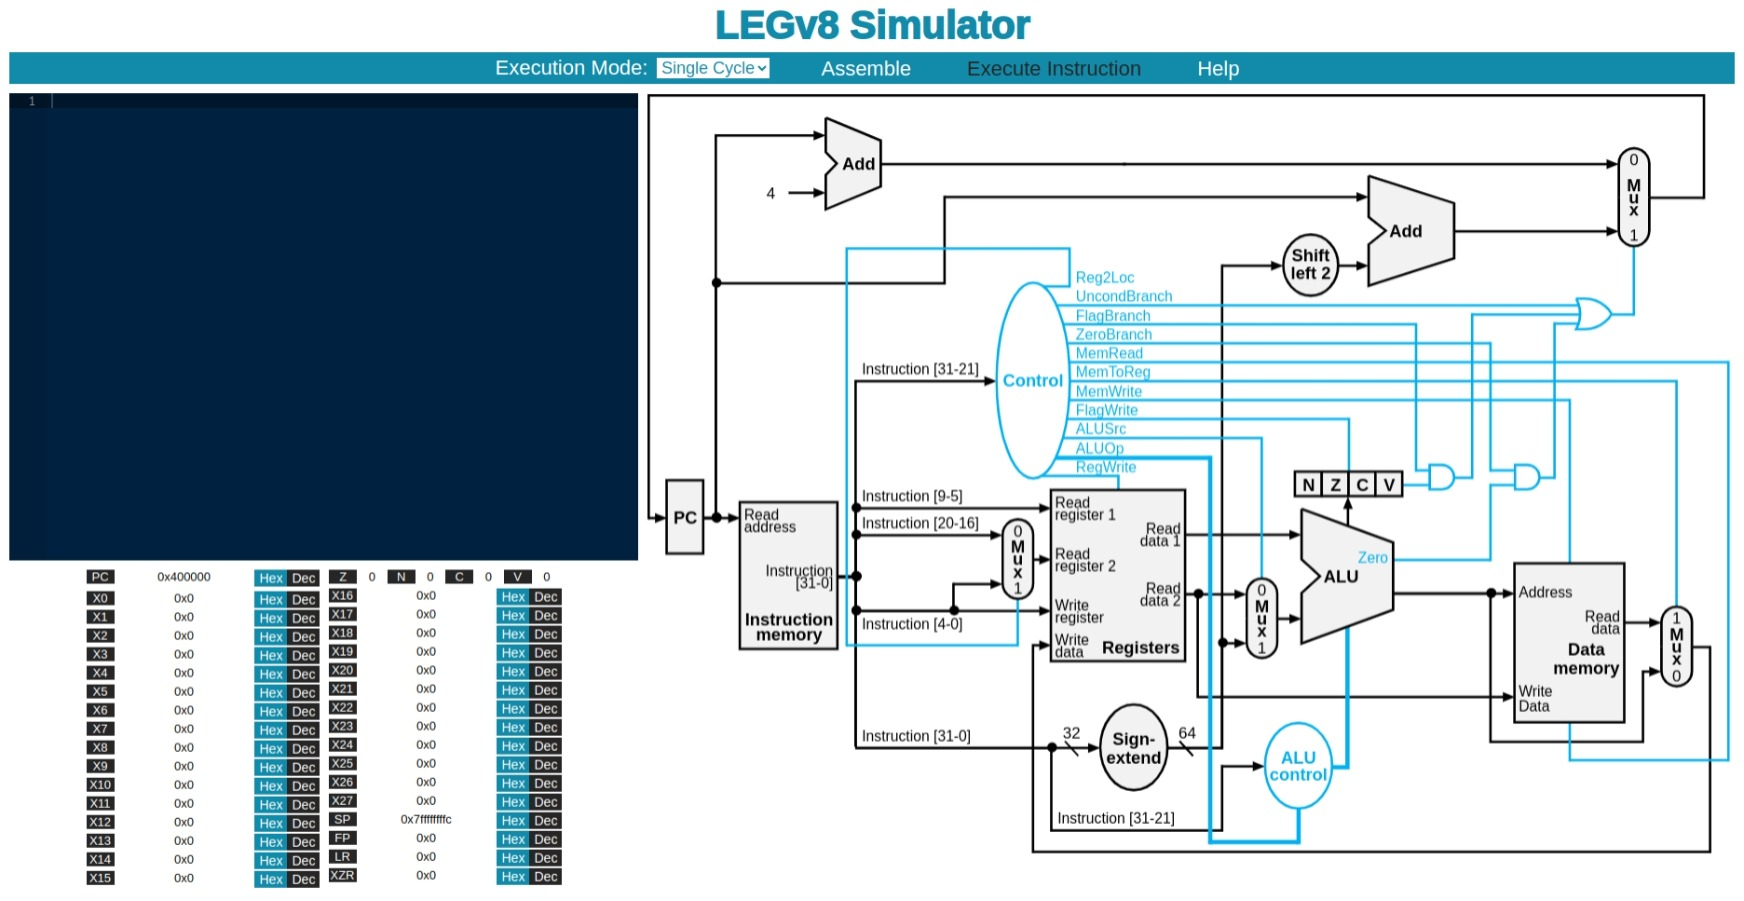
\includegraphics[width=.85\textwidth]{img/old_single_cycle.jpeg}
	}
	
	\subfigure[Pipeline]{
		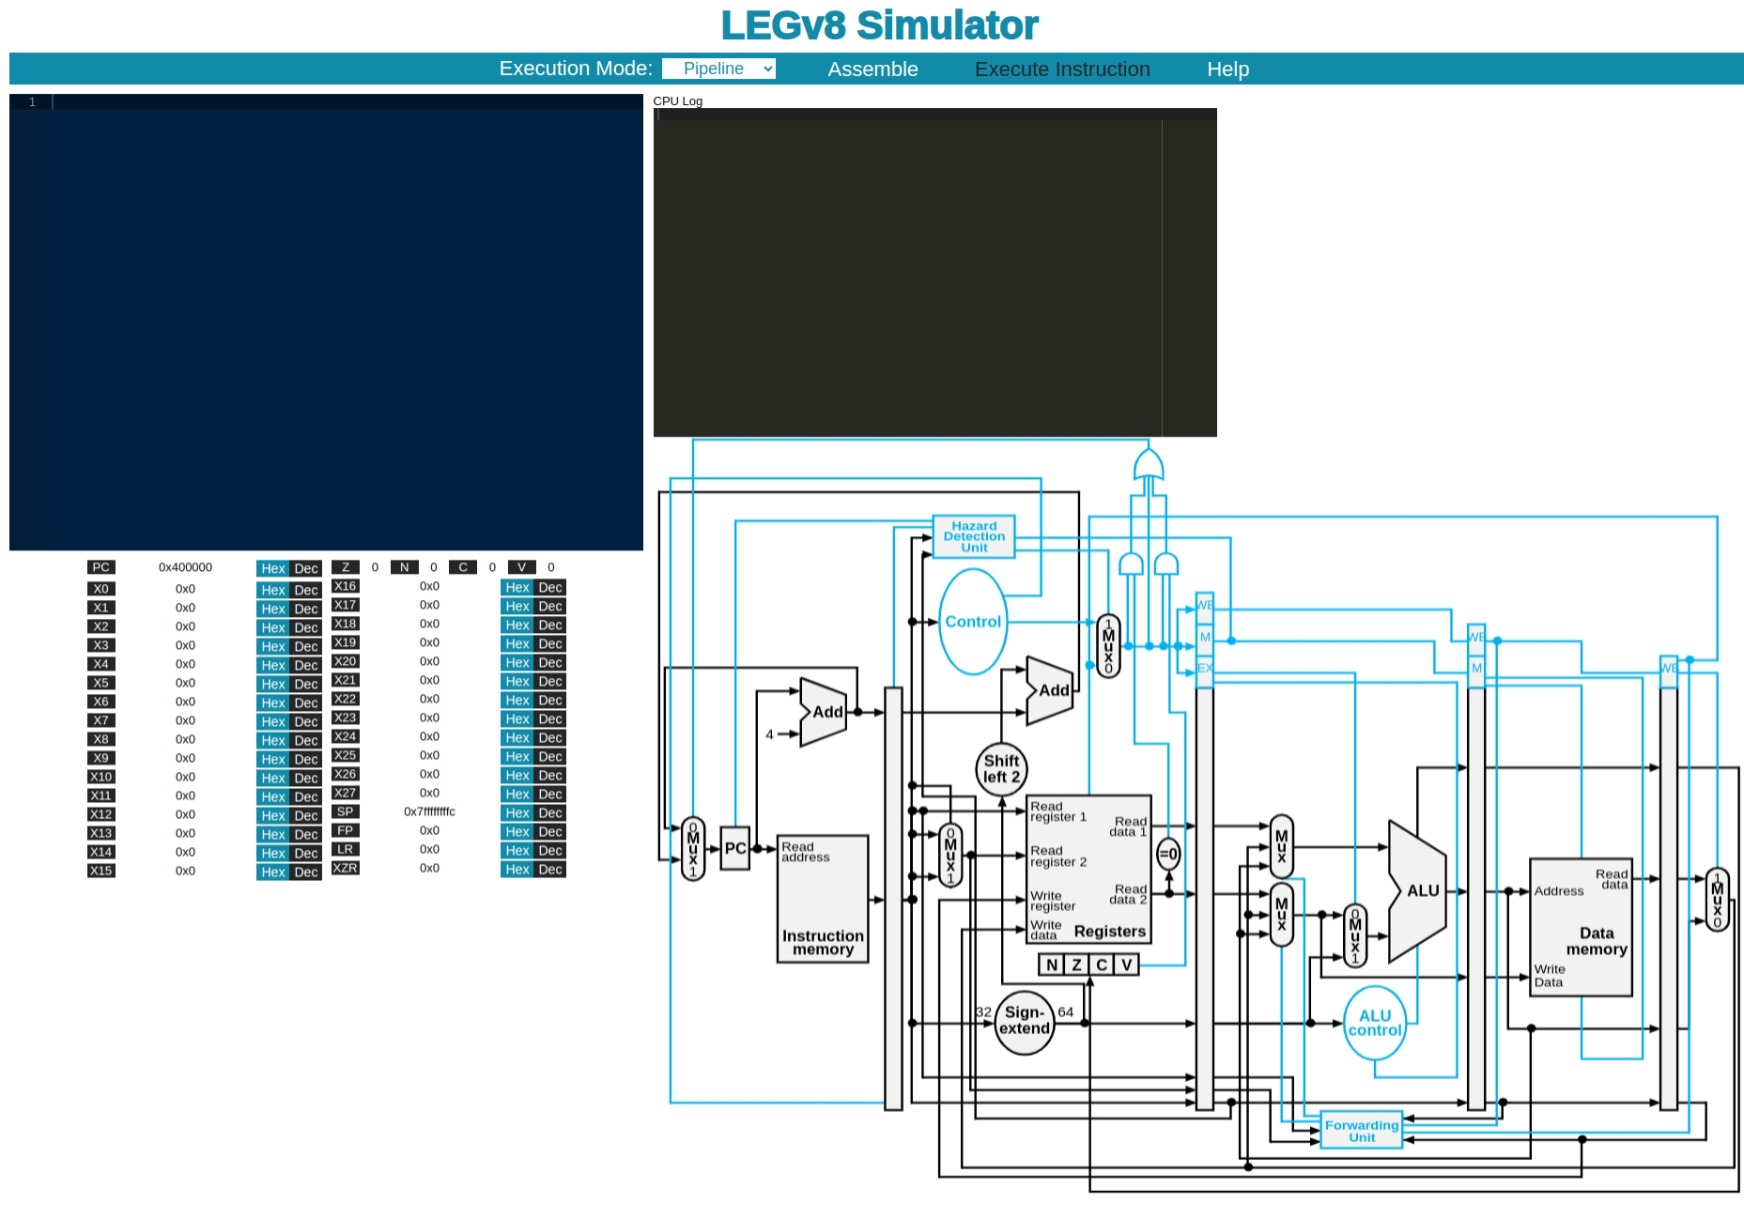
\includegraphics[width=.85\textwidth]{img/old_pipeline.jpeg}
	}
	\caption{The simulator's main page with the two different execution modes.}
\end{figure}

\subsection*{Features}

This simulator presents many favorable characteristics:

\begin{itemize}[label=\textendash]
	\item Written in Java (platform agnostic, extensible).
	\item Compiled as a web application (platform agnostic and easily deployable).
	\item Embedded text editor to input code and display errors to.
	\item Clear and rich visualization of the \verb|X| and flag registers and the datapath of the CPU thanks to the web-based interface.
	\item Almost all of the integer arithmetic is already implemented.
	\item All types of integer \verb|LOAD| and \verb|STORE| instructions are already implemented, including \verb|STXUR| and \verb|LDXUR|.
	\item Officially distributed by ARM Education (biggest support and discoverability).
\end{itemize}


\subsection*{Problems}

Unfortunately many problems present themselves when trying to run or develop the simulator:

\begin{itemize}[label=\textendash]
	\item Absence of any documentation on how to build the project and design choices behind it.
	\item Executable version distributed in automatically-generated web page form.
	\item Pipeline execution is incomplete.
	\item The mechanism for calling subroutines is broken and results in infinite loops, making it impossible to delegate code to other functions.
	\item The mechanism for performing comparisons is broken and results in the wrong branches being taken, making it impossible to perform conditional operations and loops.
	\item The project is heavily dependent on the Eclipse Java IDE with an old GWT plugin to perform the build process.
	\item The project depends on the outdated and barely supported GWT library to deploy the simulator as a web application. This restricts the developers from using newer Java features or better web frameworks.
\end{itemize}


I present below a demonstration of the bugs regarding the subroutine calls and number comparisons:

\begin{figure}[H]
	\centering
	\subfigure[BL instruction writes the incorrect address to the return register (LR)]{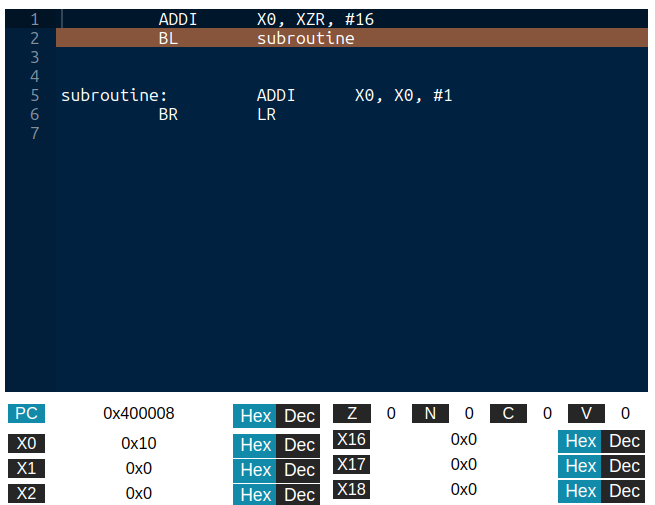
\includegraphics[width=.45\textwidth]{img/br_bug_1.png}}
	\subfigure[Jumps to the subroutine and increments X0]{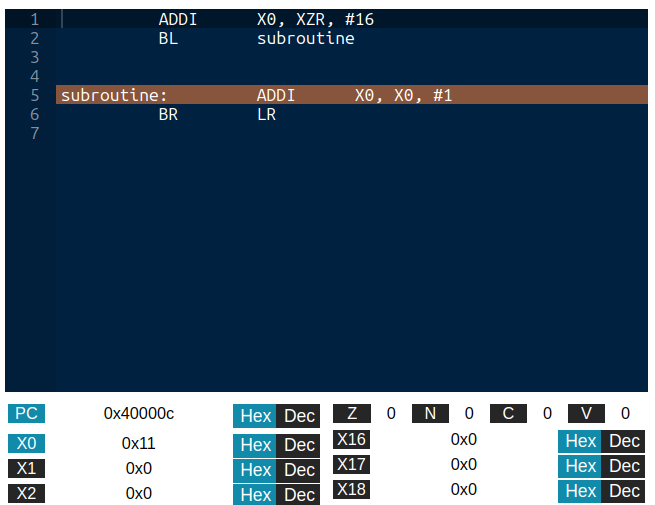
\includegraphics[width=.45\textwidth]{img/br_bug_2.png}}
	\subfigure[Reads wrong address from LR]{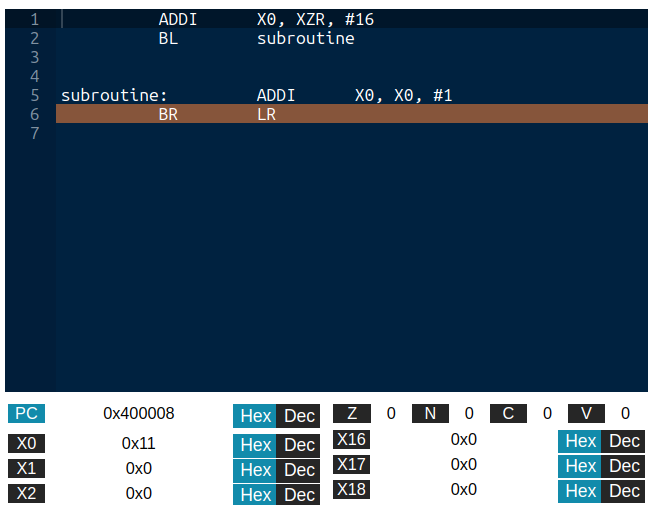
\includegraphics[width=.45\textwidth]{img/br_bug_3.png}}
	\subfigure[Returns to the start of the subroutine instead of the main program]{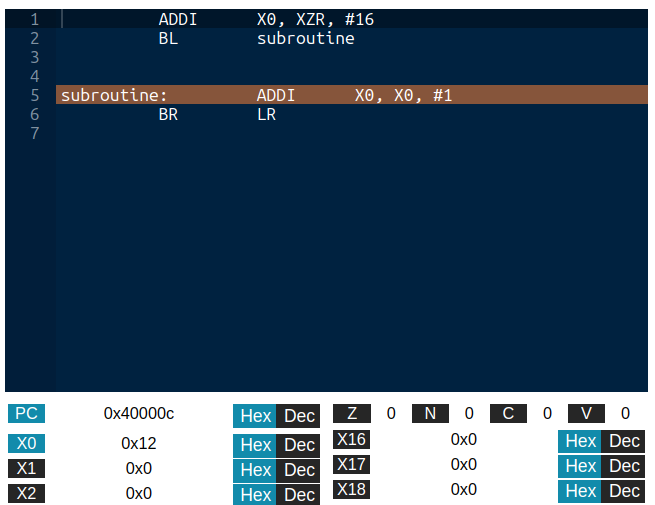
\includegraphics[width=.45\textwidth]{img/br_bug_4.png}}
	\caption{Branch returns to the wrong instruction, making it execute the branch in a loop}
\end{figure}

\begin{figure}[H]
	\centering
	\subfigure[X0 < X1]{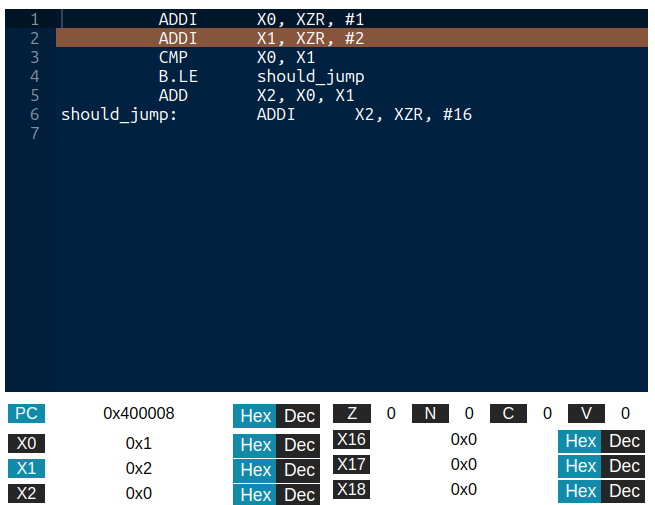
\includegraphics[width=.45\textwidth]{img/cmp_bug_1.png}}
	\subfigure[Comparison sets the flags incorrectly]{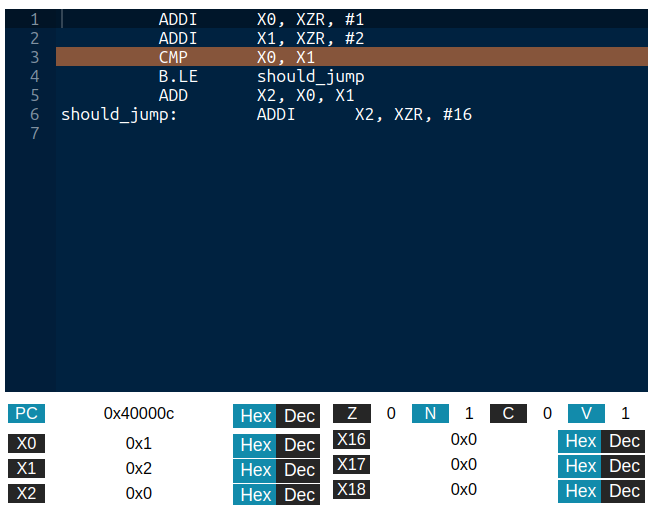
\includegraphics[width=.45\textwidth]{img/cmp_bug_2.png}}
	\subfigure[Less-or-equals jump doesn't happen]{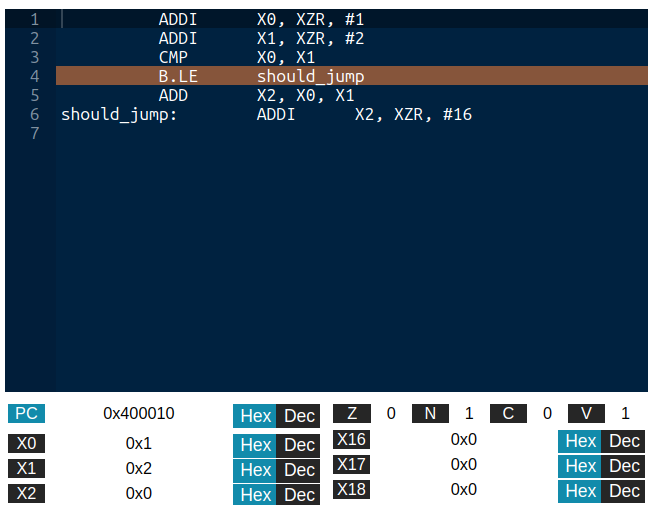
\includegraphics[width=.45\textwidth]{img/cmp_bug_3.png}}
	\subfigure[Wrong instruction executed]{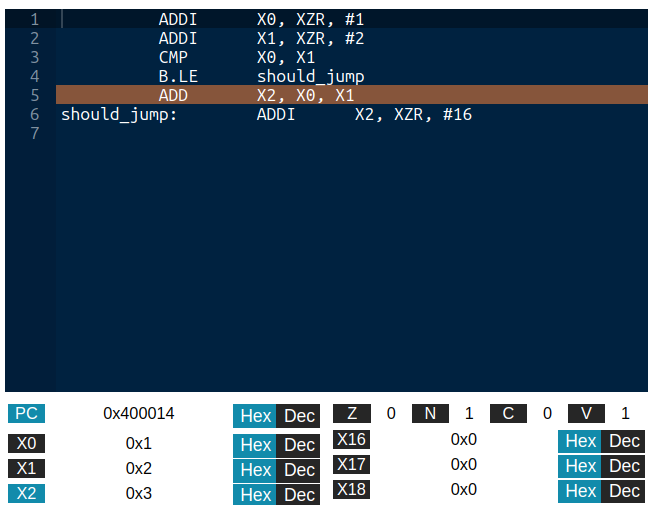
\includegraphics[width=.45\textwidth]{img/cmp_bug_4.png}}
	\caption{Comparisons do not set the correct flags and thus fail}
\end{figure}

\subsection*{Motivations}

For these reasons, this simulator was chosen as the subject of my thesis:

\begin{itemize}[label=\textendash]
	\item Maximize the impact of my work by fixing and improving the most popular simulator available
	\item Provide the first complete implementation of the LEGv8 instruction set
	\item Allow the Digital Systems Architecture course at UniTS and other courses in general to have a working LEGv8 simulator for more effective teaching
	\item Opportunity to work on a real Java code base
\end{itemize}

\subsection*{The simulator's inner workings}
\newpage
\chapter{Building and modernizing the code base}\label{chap:chap2}

\epigraph{``Much of the excitement we get out of our work is that we don't really know what we are doing''}{\textit{Edsger W. Dijkstra}}

\subsection*{Getting the project to compile}

As was pointed out in Chapter 1, the project's documentation lacks any kind of indications of how to successfully build it \footnote{\url{https://raw.githubusercontent.com/arm-university/Graphical-Micro-Architecture-Simulator/main/README.md}}.
The presence of a \verb|.project| file indicates that at some point it was developed using the Eclipse IDE \footnote{\url{https://www.eclipse.org/}}. Furthermore the existence of a \verb|.gwt.xml| file \footnote{\url{https://raw.githubusercontent.com/arm-university/Graphical-Micro-Architecture-Simulator/main/LEGv8_Simulator/src/com/arm/legv8simulator/LEGv8_Simulator.gwt.xml}} makes it clear that the GWT framework \footnote{\url{https://www.gwtproject.org/}} is being used to generate the web application. Its contents tell us that the JDK version to use is Java 8, since that's the latest GWT v2.7 (partially) supports \footnote{As we can see, until v2.8, GWT didn't even support basic Java constructs such as Map, Arrays, BigInteger, Stream, etc. \url{https://www.gwtproject.org/release-notes.html#Release_Notes_2_8_0}}. By reading the file we also discover that the project uses a module called AceGWT \footnote{\url{https://github.com/daveho/AceGWT}}, a port of an older version of the ACE editor \footnote{\url{https://ace.c9.io/}} that implement GWT bindings and allows the web application to embed a text editor. The project uses the 1.0.0 release of AceGWT \footnote{\url{https://github.com/daveho/AceGWT/releases/tag/1.0.0}} which predates its integration with Maven \footnote{Maven is a build automation system that allows to automatically fetch and import libraries to your Java project and compile and deploy it: \url{https://maven.apache.org}}.
\newline
By piecing together these clues I cloned the repository, downloaded both the GWT v2.7 and AceGWT's 1.0.0 releases and imported the project into Eclipse. GWT's website also suggests using GWT's Eclipse plugin \footnote{\url{https://www.gwtproject.org/usingeclipse.html}}, so that was installed as well.
\newline
The project expected to have access to some files and libraries in certain places, so by configuring correctly the build path of the project I was able to get it to finally compile \footnote{The entire process is available as a PDF file or static web page: \url{https://github.com/arm-university/Graphical-Micro-Architecture-Simulator/pull/7}}.
\newline
This set-up allowed me to do most of the work presented in this thesis, but presented a few glaring problems when thinking about the future maintainability of the software:

\begin{itemize}
	\item Changes to the Eclipse IDE introduced after version 2023-09 have made it impossible to install the GWT plugin. This means that any future development would need to happen on an old version of the IDE unless an official fix was provided.
	\item Both AceGWT and GWT have switched to Maven in their latest releases, making the importing, dependency management, and building of the code base automatic.
	\item The project uses an old version of GWT and could make use of the new features implemented in the newer releases.
	\item Downloading the dependencies and manually setting up the project from a non-working state each time is a tedious and finnicky process that cannot be depended upon in case something changes to the IDE.
	\item The project is forever bounded to the Eclipse IDE, meaning it cannot be automatically built headlessly through a script or developed using more modern and featureful IDEs.
	\item The building process is not well configured. For example, it's not possible to change the directory where the web application is compiled and all the web resources need ot be already present in the output folder otherwise the web application cannot be launched. 
\end{itemize}

Thus, my aim was to make the project as agnostic as possible and turn the set-up into a 1-click process to make it viable for future developers to get started collaborating without any roadblocks. This has been mostly achieved by porting the project to Maven, and in the process making a few updates to the environment.

\subsection*{Modernizing the project and porting to Maven}

This part of my work progressed through much trial and error. After reading through the Maven and GWT documentation and creating empty GWT projects using their newest tools, I figured out how to configure Maven's \verb|pom.xml| and GWT's \verb|.gwt.xml| files to correctly import the latest version of GWT and make it recognize the project as a GWT web application. As part of the modernization, I created a local Maven repository in which I built a custom version of AceGWT using the latest version of GWT. Lastly, even though GWT still doesn't support the entirety of Java 8, it is possible to use JDK 21 to build the project and utilize some newer Java features in the code.
\newline
After all of this was done, downloading, configuring, and building the project was reduced to running \verb|git clone| and \verb|mvn package| inside the project's directory when using the command line. This also made it possible to import and develop the project on any Java IDE that supports Maven by doing the same steps using the IDE's graphical workflow.
\newpage
\chapter{Bug fixing and new features}\label{chap:lipsum}

\epigraph{``If debugging is the process of removing software bugs, then programming must be the process of putting them in.''}{\textit{Edsger W. Dijkstra}}

\subsection*{Getting the project to a working state}

\paragraph*{The flag setting bug}

In LEGv8, CMP and CMPI are pseudoinstructions, meaning that under the hood they actually make use of the SUBS and SUBIS instructions respectively to set the compare flags. The fact that the former instructions failed, pointed at a problem in the latter ones, which was proven to be correct. The simulator first implements the function responsible for setting the flags of the addition operations and when setting the flags for the subtraction operations it simply calls the same function with the same arguments.
\begin{lstlisting}[caption={The adddition flag-setting code}]
	private void ADDSetFlags(long result, long op1, long op2) {
		setNflag(result < 0);
		setZflag(result == 0);
		setCflag(result, op1, op2);
		setVflag(result, op1, op2);
	}
\end{lstlisting}
\begin{lstlisting}[caption={The buggy subtraction flag-setting code}]
	private void SUBSetFlags(long result, long op1, long op2) {
		ADDSetFlags(result, op1, op2);
	}
\end{lstlisting}
As we can see, this presents a problem since subtraction and addition set their flags in a different way. The fix was simply to call the same function but with the 2-complement of the second operand.
\begin{lstlisting}[caption={The fixed subtraction flag-setting code}]
	private void SUBSetFlags(long result, long op1, long op2) {
		ADDSetFlags(result, op1, (~op2)+1);
	}
\end{lstlisting}

\paragraph*{The branch return bug}

For this bug, inspecting the LR register showed that the BL instruction was not writing the register with the address of the current instruction, but with the subroutine's one instead. This created an infinite loop since, when the subroutine returned to the LR, the program would jump back to the beginning of the subroutine all over again.
\begin{lstlisting}[caption={The buggy address writing}]
	private void BL(int branchIndex) {
		instructionIndex = branchIndex;
		XRegisterFile[LR].writeDoubleWord(instructionIndex * INSTRUCTION_SIZE + Memory.TEXT_SEGMENT_OFFSET);
		...
	}
\end{lstlisting}
As we can see, the instructionIndex is updated too soon and thus the LR register gets written with the address of the branch.
\begin{lstlisting}[caption={The fixed address writing}]
	private void BL(int branchIndex) {
		XRegisterFile[LR].writeDoubleWord(instructionIndex * INSTRUCTION_SIZE + Memory.TEXT_SEGMENT_OFFSET);
		instructionIndex = branchIndex;
		...
	}
\end{lstlisting}

\paragraph*{The datapath visualization bug}
An issue that was raised on GitHub \footnote{\url{https://github.com/arm-university/Graphical-Micro-Architecture-Simulator/issues/8}} complained about erroneous values of the MemWrite and MemRead signals from the control unit. This was a problem in the configuration.
\begin{lstlisting}[caption={Buggy SingleCycleVis.java}]
	...
	ctx.fillText(ControlUnitConfiguration.toString(c.memRead), DATA_MEM_COORDS[0]+DATA_MEM_DIMENSIONS[0]/2-t.getWidth()-1, DATA_MEM_COORDS[1]-3);
	ctx.fillText(ControlUnitConfiguration.toString(c.memToReg), MUX_READ_DATA_MEM_COORDS[0]+MUX_READ_DATA_MEM_DIMENSIONS[0]/2-t.getWidth()-1, MUX_READ_DATA_MEM_COORDS[1]-3);
	ctx.fillText(ControlUnitConfiguration.toString(c.memRead), DATA_MEM_COORDS[0]+DATA_MEM_DIMENSIONS[0]/2-t.getWidth()-1, DATA_MEM_COORDS[1]+DATA_MEM_DIMENSIONS[1]+10);
	...
\end{lstlisting}
\begin{lstlisting}[caption={Fixed SingleCycleVis.java}]
	...
	ctx.fillText(ControlUnitConfiguration.toString(c.memWrite), DATA_MEM_COORDS[0]+DATA_MEM_DIMENSIONS[0]/2-t.getWidth()-1, DATA_MEM_COORDS[1]-3);
	ctx.fillText(ControlUnitConfiguration.toString(c.memToReg), MUX_READ_DATA_MEM_COORDS[0]+MUX_READ_DATA_MEM_DIMENSIONS[0]/2-t.getWidth()-1, MUX_READ_DATA_MEM_COORDS[1]-3);
	ctx.fillText(ControlUnitConfiguration.toString(c.memRead), DATA_MEM_COORDS[0]+DATA_MEM_DIMENSIONS[0]/2-t.getWidth()-1, DATA_MEM_COORDS[1]+DATA_MEM_DIMENSIONS[1]+10);
	...
\end{lstlisting}
\begin{lstlisting}[caption={BuggyControlUnitConfiguration.java}]
	...
	RM_LOAD(null, false, false, false, false, true, true, false, true, 0, true),
	...
\end{lstlisting}
\begin{lstlisting}[caption={Fixed ControlUnitConfiguration.java}]
	...
	RM_LOAD(null, false, false, false, true, true, false, false, true, 0, true),
	...
\end{lstlisting}

\subsection*{Adding new features}

\paragraph{Refactoring the memory}

The \verb|ByteBuffer.java| and \verb|Memory.java| classes have mostly been left untouched, although their methods and variables presented some Java-centric names and have thus been replaced with more apt LEGv8 names such as \verb|getDoubleWord| instead of \verb|getLong|. The base address of the stack, defined in the textbook as \verb|0x7ffffffffc|,  was not quadword-aligned, leading to a design contradiction. I chose to change it to the  compatible address \verb|0x8000000000|.

\paragraph{Completing the integer arithmetic}

The integer-related instructions missing from the simulator were: \verb|MUL|, \verb|SMULH|, \verb|UMULH|, \verb|SDIV|, and \verb|UDIV|. In order to implement these new instructions a few changes to the code had to be made. First of all they had been added to \verb|Mnemonic.java|.
\begin{lstlisting}[caption={}]
	...
	...
\end{lstlisting}
\begin{lstlisting}[caption={Added mnemonics}]
	...
	MUL("MUL", "mul", TokenType.XMNEMONIC_RRR, "10011011000", "0010"),
	SMULH("SMULH", "smulh", TokenType.XMNEMONIC_RRR, "10011011010", "0010"),
	UMULH("UMULH", "umulh", TokenType.XMNEMONIC_RRR, "10011011110", "0010"),
	SDIV("SDIV", "sdiv", TokenType.XMNEMONIC_RRR, "10011010110", "0010")
	UDIV("UDIV", "udiv", TokenType.XMNEMONIC_RRR, "10011010110", "0010"),
	...
\end{lstlisting}
Then to Decoder.java
\begin{lstlisting}[caption={Added instructions to the decoder}]
	...
	case MUL :
	return new Instruction(mnemonic, decodeRRRArgs(args), lineNumber, ControlUnitConfiguration.RRR);
	case UMULH :
	return new Instruction(mnemonic, decodeRRRArgs(args), lineNumber, ControlUnitConfiguration.RRR);
	case SMULH :
	return new Instruction(mnemonic, decodeRRRArgs(args), lineNumber, ControlUnitConfiguration.RRR);
	case UDIV :
	return new Instruction(mnemonic, decodeRRRArgs(args), lineNumber, ControlUnitConfiguration.RRR);
	case SDIV :
	return new Instruction(mnemonic, decodeRRRArgs(args), lineNumber, ControlUnitConfiguration.RRR);
	...
\end{lstlisting}
Then they had to be added to \verb|TokenType.java| to use with the parser
\begin{lstlisting}[caption={Addition to the parser}]
	...
		MNEMONIC_RRR("ADDS?[ \t]+|SUBS?[ \t]+|ANDS?[ \t]+|MUL[ \t]+|SMULH[ \t]+|UMULH[ \t]+|SDIV[ \t]+|UDIV[ \t]+|ORR[ \t]+|EOR[ \t]+|adds?[ \t]+|fmul[sd]?[ \t]+|fdiv[sd]?[ \t]+|subs?[ \t]+|ands?[ \t]+|mul[ \t]+|smulh[ \t]+|umulh[ \t]+|sdiv[ \t]+|udiv[ \t]+|orr[ \t]+|eor[ \t]+", 15, "MNEMONIC"),
	...
\end{lstlisting}
And finally they had to be implemented inside \verb|CPU.java| to execute the operations
\begin{lstlisting}[caption={}]
	...
	private void MUL(int destReg, int op1Reg, int op2Reg) {											
			XRegisterFile[destReg].writeDoubleWord(XRegisterFile[op1Reg].readDoubleWord() * XRegisterFile[op2Reg].readDoubleWord());
		}
	}
	private void SDIV(int destReg, int op1Reg, int op2Reg) {
			XRegisterFile[destReg].writeDoubleWord(XRegisterFile[op1Reg].readDoubleWord() / XRegisterFile[op2Reg].readDoubleWord());
	}
	
	private void UDIV(int destReg, int op1Reg, int op2Reg) {
			BigInteger dividend = BigInteger.valueOf(XRegisterFile[op1Reg].readDoubleWord()).and(UNSIGNED_LONG_MASK);
			BigInteger divisor = BigInteger.valueOf(XRegisterFile[op2Reg].readDoubleWord()).and(UNSIGNED_LONG_MASK);
			BigInteger quotient = dividend.divide(divisor);
			XRegisterFile[destReg].writeDoubleWord(quotient.longValue());
	}
	
	private void SMULH(int destReg, int op1Reg, int op2Reg) {
			BigInteger fullResult = BigInteger.valueOf(XRegisterFile[op1Reg].readDoubleWord()).multiply(BigInteger.valueOf(XRegisterFile[op2Reg].readDoubleWord()));
			BigInteger shiftedResult = fullResult.bitLength() > 64 ? fullResult.shiftRight(64) : BigInteger.valueOf(0);
			XRegisterFile[destReg].writeDoubleWord(shiftedResult.longValue());;
			
	}
	
	private void UMULH(int destReg, int op1Reg, int op2Reg) {
			BigInteger fullResult = BigInteger.valueOf(XRegisterFile[op1Reg].readDoubleWord()).and(UNSIGNED_LONG_MASK).multiply(BigInteger.valueOf(XRegisterFile[op2Reg].readDoubleWord()).and(UNSIGNED_LONG_MASK));
			BigInteger shiftedResult = fullResult.bitLength() > 64 ? fullResult.shiftRight(64) : BigInteger.valueOf(0);
			XRegisterFile[destReg].writeDoubleWord(shiftedResult.longValue());;
	}
	...
\end{lstlisting}
Of particular interest are the \verb|UDIV|, \verb|UMULH| and \verb|SMULH| instructions as they make use of the \verb|BigInteger| class.
\begin{itemize}[label=\textendash]
\item Java does not support unsigned integers. This means that \verb|UDIV| needs to artificially represent them with 65 bit signed numbers through the use of a bit mask. This way it's able to perform the division and return a native 64 bit signed integer.
\item The \verb|*MULH| instructions perform a 128-bit multiplication between two 64-bit integers and retain the higher 64 bits. To perform such a calculation Java needs to go beyond its primitive types and make use of \verb|BigInteger|.
\end{itemize}
Of course this could have been done in more primitive ways through the use of arrays, but GWT supported the \verb|BigInteger| type and allowed to solve the problem quickly.

\paragraph*{Visualizing the stack}

After finishing implementing the integer arithmetic it was time to make the stack visible inside the web interface. This was done by reutilizing the same structure that allowed for the visualization of the \verb|X| registers and slightly tweaking it for memory usage by .

\paragraph*{Implementing floating point arithmetic}
\subparagraph*{Adding floating point registers}
\subparagraph*{Adding floating point operations}
\subparagraph*{Visualizing the new registers}
\subparagraph*{Visualizing the data path}
\newpage
\chapter{Current problems and further development}\label{chap:chap4}

\epigraph{``Perfecting oneself is as much unlearning as it is learning.''}{\textit{Edsger W. Dijkstra}}



\subsection*{Current shortcomings and proposals}

Here is a list of things that can be fixed or added without fundamentally changing how the project is structured:

\begin{itemize}
	\item The pipelined execution does not work properly, especially with the newly introduced floating point operations. This is because the code modeling the CPU is not logically divided into the pipeline stages and makes it difficult to run and synchronize multiple instructions at a time. This can be done by reorganizing the project's code to make it follow closer to the 5 stages of the LEGv8 pipeline.
	\item Even though the project is written in Java, it makes many design decisions that don't make use of the power of object-orientation. It doesn't properly divide the components of the ISA into their own classes, it presents many code repetitions and doesn't use many abstractions, and in general some classes and methods are disproportionally large. The code base should be refactored using the latest design principles of Java's object-oriented programming and make use of the additions that GWT has implemented from v2.7 onwards.
	\item The project lacks any code testing capabilities. Tests should be written using Maven's convention in order to make sure the simulator works correctly and to avoid breaking changes in the future.
	\item The project currently has to include a custom-compiled version of AceGWT as a local repository. This can be fixed by either:
	\begin{itemize}[label=$\rightarrow$]
		\item Uploading this custom version to Maven's central repository.
		\item Configuring Maven and using some plugins in order to use AceGWT's GitHub repository as a Maven repository and automatically apply the patches and build the custom version of the library on the fly.
	\end{itemize}
	\item Make the web UI more responsive and change its layout to work better on devices with smaller screens. In general, improve the look and feel of the application.
	\item Currently, code can only be executed by manually stepping over the instructions. A way of automatically running all the code until completion or stepping automatically with a user-defined clock speed could be helpful when trying to test results faster.
	\item The project lacks documentation. More code comments should be written and a more thorough description of the simulator's design and functionalities should be provided both to users and to developers. This thesis could be a start.
\end{itemize}

\subsection*{Structural problems}

These are the problems I found with the simulator that, should they be fixed, would require a lot of work and would change the code base in a fundamental way.

\begin{itemize}
 	\item The textbook doesn't really specify the logical implementation of the ISA for anything other than a few integer instructions. This means that, for example, things like ALUop codes are not defined for floating point operations. In order to provide a complete simulation of the LEGv8 ISA, some arbitrary design decisions should be made to extend Patterson's and Hannessy's work.
 	\item Similarly, the texbook doesn't talk about pipelined execution in the context of floating point operations. This means that implementing it would require the programmer to make its own informed design decisions.
 	\item Java does not allow data structured to contain more than $2^{32}$ elements. This means that things such as the main memory cannot be properly simulated with a single data structure, but a tiered approach should be taken. Of course this is a very minor problem, since LEGv8 is purely for educational usage and realistically no program using more than a moderate amount of memory and instructions will be written.
 	\item If the application needs to be deployed and ran in the browser as a web application, replacing GWT could be considered. It's a very old library that has stopped being officially supported by Google long ago \footnote{\url{https://en.wikipedia.org/wiki/Google_Web_Toolkit}} and cannot keep up with the new features of both the Java language and the web. A new framework for creating self-contained web applications with Java should be identified and the project rewritten to make use of it. Unfortunately, GWT's main advantage is the ability to write Java code and have it seamlessly transpiled to JavaScript, whereas most frameworks use Java only for the back end and require the programmer to write the client-side logic in JavaScript. If no such alternative framework exists, modernizing the code base as much as possible within GWT's constraints or surveying other programming languages  could be taken into consideration. Alternatively, thanks to the portability of Java, a native UI could be written and the simulator distributed through a \verb|.jar| executable.
\end{itemize}

\newpage

%*******************************************************
% Conclusions
%*******************************************************
\chapter*{Concluding remarks}
% Do not modify this part
\addcontentsline{toc}{chapter}{Conclusions}
\label{chap:concl}
\markboth{CONCLUSIONS}{CONCLUSIONS}
% Do not modify this part

This thesis' work has consisted in analizing ARM Education's official LEGv8 simulator, bringing it up to an acceptable working state and extending it by implementing the entirety of the LEGv8 ISA and improving its general functioning and UI. As of this date, this is the only publicly available simulator to offer a complete implementation of LEGv8 and a comprehensive visualization of the stack, all of the registers, and the step-by-step state of execution.


\newpage

\backmatter

%*******************************************************
% Bibliography
%*******************************************************
\nocite{*}
\bibliography{Bib/Bibliography}
\bibliographystyle{plain}

%*******************************************************
% Final dedications and acknowledgements
%*******************************************************
% Do not modify this part
\chapter*{}
\thispagestyle{empty}
\vspace*{3cm}
% Do not modify this part

\begin{center}
\hfill Ei fu. Siccome immobile, \\
\hfill Dato il mortal sospiro, \\
\hfill Stette la spoglia immemore \\
\hfill Orba di tanto spiro \\ \medskip
\hfill Alessandro Manzoni -- \emph{Il Cinque Maggio}
\end{center}

\end{document}